

\chapter{Basics}

In this background chapter, we review the statistical and probabilistic methodologies .
The goal of this chapter is to provide the basic information regarding Bayesian methods of machine learning used in the thesis. A good introduction to the field can be found in books of \cite{bishop2007pattern}, \cite{kruschke2014doing} and \cite{lee2014bayesian} . 

\section{Bayesian Model Learning}

Bayesian models are represented as probability distributions. Probability is used to quantify "uncertainty" or "Degree of belief". The models are initialized with some prior probabilities(beliefs). The observed data are used to update the prior beliefs to become posterior beliefs.

We can explain this with an example. Assume we have a bag with 50 marbles with 2 colours, red and blue. We randomly take 10 marbles out of the bag and observe their colour with replacement. What we have to model is, our belief of the numbers of colours inside the bag, in Bayesian  terms colour distribution in the bag, which we can define as $\theta$ . We cannot directly observe the bag. All that we can observe are the colours of the 10 picked marbles.

Before we do anything else we need to specify our prior belief with respect to the colour distribution $\theta$ . This belief needs to be expressed as a probability distribution, called the \emph{prior distribution}. A reasonable "prior distribution" denoted by $p(\theta)$ is one which takes uniform value between 0 and 1. Lets assume $p(\theta)$ is belief of red marbles in bag then $1 - p(\theta)$  is the belief of blue marbles in the bag. This uniform distribution is shown as dotted line in the figure 

Now we consider the observed colour of the 10 marbles from the bag. We observe 8 red marbles and 2 blue marbles. After observing the data, the updated knowledge about $\theta$ is described by a \emph{posterior distribution}, denoted by $p(\theta | D)$, where D indicates the observed data. The distribution represents the updated belief after observing the colour picked marbles. Bayes rule specifies how we can combine the information from the data, that is how to determine the posterior distribution $p (\theta | D)$ using  the prior distribution $p(\theta)$ and the likelihood  $p (D | \theta)$ :
\begin{equation}
	p(\theta | D) = \frac{p(D | \theta) p(\theta)}{p(D)}
\end{equation}

The equation is often verbalized as :
\begin{equation}
	posterior = \frac{likelihood * prior}{marginal likelihood}
\end{equation}

We note here that the posterior distribution is a combination of the prior information we had and what we have learned from the data. 



\missingfigure{Image of the prior posterior}


\section{Distributions }

The basic idea of Bayesian analysis is that quantifying the \emph{state of belief} or the \emph{state of uncertainty}, about the variables of interest. These variable(latent and observed) are always represented by probability distributions. In this thesis we exhaustively use the Dirichlet, Categorical and Bernoulli distributions. 
 
\subsection*{Dirichlet distribution}
The Dirichlet distribution is part of the exponential family. It has finite dimensional sufficient statistics. It is conjugate to the multinomial and categorical distribution. 

\subsection*{Categorical distribution}
\todo[inline]{Explain}

\subsection*{Bernoulli distribution}
\todo[inline]{Explain}
Bernoulli distribution is used when there are a number of iterations of some activity, where each iteration (or observation) may turn out to be a "success" or a "failure". From the data on T observations, we want to estimate the probability of "success"


\section{Graphical Models}

\todo[inline]{formal lingua franca for probabilistic Bayesian modelling}
Graphical models is a method to visualize complete and interpretable representation of a Bayesian probabilistic model. The nodes in the graph represent variables of the problem, and the edges connecting them represents dependencies. The graph structure is used to indicate dependencies between the variables, with children depending on their parents. The plates are used to indicate replication. We use the conventions of representing unobserved variables without shading and observed variables with shading.

\missingfigure{graphical model of above mentioned example}


\section{Probabilistic Programming Languages}

Probabilistic programming languages(PPL) are new languages developed to program probabilistic graphical models and to run inference in them. 
Until recently, Bayesian Model learning have been limited in scope, and have been hard to apply to many real-world applications. Probabilistic programming is a new approach which makes Bayesian learning easier to build and more applicable. 


\begin{figure}[htp]
\centering
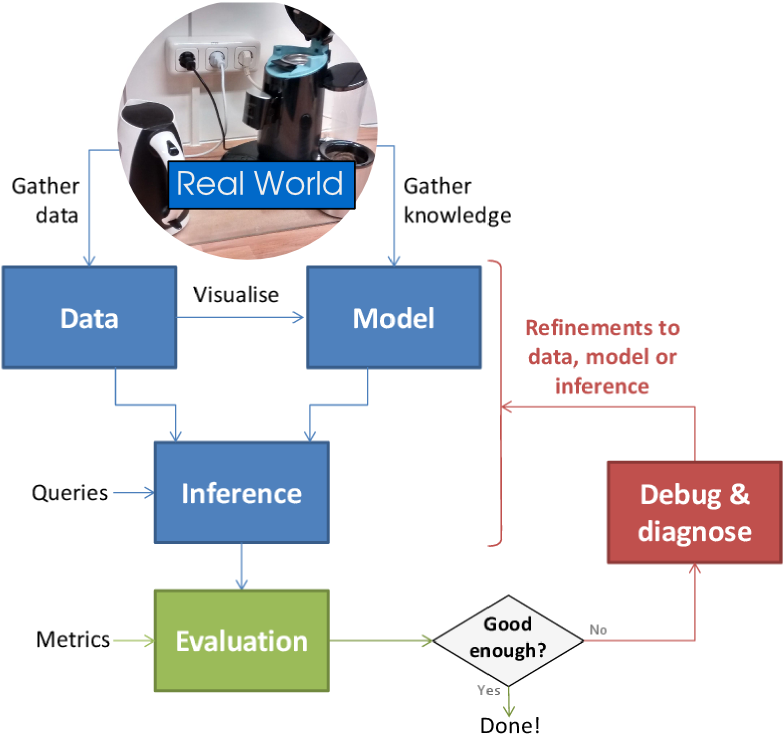
\includegraphics[width=0.8\textwidth]{pictures/Lifecycle.png}
\caption[Steps involved in probabilistic modelling ]{Steps involved in probabilistic modelling  \protect\footnotemark }
\label{}
\end{figure}

\footnotetext{\url{ http://www.mbmlbook.com/LifeCycle.html}}
\textbf{Probabilistic Programming} gives us a framework in which we can create any model, based on our assumptions of the process. The model is basically expressing the assumptions in a mathematical form. The assumptions are the number of variables in the model, the relation between these variables, changes in which variables affects which other variables. This model is then used to generate a problem specific algorithm which can be used to solve the machine learning problem in hand. 

\subsection*{Steps required in Probabilistic Modelling}
\label{sub:steps}
\begin{enumerate}
	\item \textbf{Gather data} to be used for training and evaluation.
    \item \textbf{Gather knowledge} required for model building.
    \item \textbf{Visualise} the data to understand it. This is useful also for gathering knowledge. After visualization the insight gained can be used for assumptions in model building.
    \item \textbf{Construct a model} based on the knowledge of the problem statement available and data visualization. 
    \item \textbf{Perform inference} using both the data and the constructed model. The variables of the model are tuned based on the data available. Predictions can be made to find out the knowledge gained by the model.
    \item \textbf{Evaluate} the performance of the model based on evaluation metric.
    \item \textbf{Diagnose} the model and the assumptions if the evaluation is below some acceptable range
    \item \textbf{Refine the system} by adapting different model structure, inference engine

\end{enumerate}
% subsection steps (end)


The separation of the model choices and the inference engine for generating machine algorithms have given rise to a new kind of programming language.
In the software framework you need to provide the description of your model and the selection of the inference engine, which internally produces the code for the machine learning algorithm.
Examples of software frameworks that implement the probabilistic modelling philosophy  include CHURCH \cite{goodman_church_2012}, Venture \cite{mansinghka_venture_2014}, PyMC3 \cite{salvatier_probabilistic_2015}, BayesPy \cite{luttinen_bayespy_2014} and Infer.net \cite{minka_2010}.

\subsection{PyMC3}

\textbf{PyMC3} is python module for Bayesian modelling. It provides intuitive model specification syntax for designing the models. The inference is primarily focussed on advanced Markov chain Monto Carlo fitting algorithms.


\subsection{BayesPy}

\textbf{BayesPy} provides tools to do Bayesian modelling. In BayesPy users construct their models, observes data and then runs inference. The inference engine present in BayesPy is variational Bayesian inference.

\subsection{WebPPL}

\textbf{WebPPL} is a javascript module for Bayesian modelling. The inference is using Markov chain Monto Carlo algorithms. Its particularly useful for doing learning inside web based database like MongoDB.

\section{Notation and terminology}
Throughout the thesis, we are referring to entities such as ``locations," ``hours," and ``observations".
This helps to guide intuition and maintain continuity of thoughts as we guide through related problems involving collections of data.
Formally we define the following terms:
\begin{itemize}
	\item A \emph{location} is the basic unit of the discrete data, defined to be an item from a set of locations. These locations can be rooms of the home or different compartments of the kitchen. 
	\item An \emph{period} is a sequence of $N$ locations denoted by $\textbf{p} = {x_1;x_2;:::;x_N}$. These represents the locations observed in a particular period of time.
	\item A \emph{observations} is a collection of $T$ periods denoted by $ D = {p_1;p_2;:::;p_T}$. These represents the complete data collected by the robot.
\end{itemize}


We also use the entities such as ``data," ``information," and ``knowledge" throughout the thesis. These can be define as:
\begin{itemize}
	\item A \emph{data} corresponds to sensor output. All the output of the sensors recorded by the robot is a data. For example RGB image from a camera, depth points from depth sensors etc.
	\item A \emph{information} corresponds to output of algorithms which process on the above data. For example vision algorithms process RGB images data to extract information of objects or persons in the image.
	\item A \emph{knowledge} corresponds to output of algorithms which process on the above information. For example vision algorithms can process detected object information in consecutive RGB frames to extract knowledge that the object was moving.
\end{itemize}
